\documentclass[conference]{IEEEtran}
\IEEEoverridecommandlockouts

\usepackage{cite}
\usepackage{amsmath,amssymb,amsfonts}
\usepackage{algorithmic}
\usepackage{graphicx}
\usepackage{textcomp}
\usepackage{xcolor}
\usepackage{array}
\usepackage{url}
\usepackage{tikz}
\usetikzlibrary{shapes.geometric, arrows.meta, positioning}

\begin{document}
	
	\title{Original Method: Deep Learning-Based Crater Detection in Lunar Imagery}
	
	\author{\IEEEauthorblockN{Scott Nguyen}
		\IEEEauthorblockA{\textit{Department of Electrical and Computer Engineering} \\
			\textit{University of New Mexico}\\
			Albuquerque, USA \\
	}}
	
	\maketitle
	
	\begin{abstract}
		This project focuses on detecting impact craters in high-resolution lunar imagery using deep learning-based object detection methods. The proposed system uses real Lunar Reconnaissance Orbiter Camera (LROC) Narrow Angle Camera (NAC) images collected from multiple lunar regions and constructs bounding-box ground truth annotations for crater instances. The project compares multiple modern detection paradigms, including one-stage detectors, two-stage detectors, and crater-detection-specific deep learning methods from the literature. Performance will be evaluated using object detection metrics such as Intersection over Union (IoU), precision, recall, and mean Average Precision (mAP). In addition to model comparison, the project emphasizes dataset construction, annotation consistency, and practical evaluation under realistic lunar imaging conditions.
	\end{abstract}
	
	\begin{IEEEkeywords}
		crater detection, lunar imagery, object detection, deep learning, LROC, bounding boxes, planetary image analysis
	\end{IEEEkeywords}
	
	\section{Introduction}
	Accurate detection of impact craters in planetary imagery is an important problem in planetary science, with applications in geological analysis, surface age estimation, terrain understanding, and mission planning. Craters are among the most common surface structures on the Moon, and automated crater detection can support large-scale analysis that would be difficult to perform manually.
	
	Traditional approaches to crater detection have relied on classical image processing techniques such as edge detection, thresholding, region analysis, and circular Hough transforms. Although these methods can work under controlled conditions, they often struggle with realistic lunar imagery because crater appearance varies with illumination, terrain texture, erosion, partial overlap, and viewing conditions.
	
	Recent deep learning methods have provided more robust alternatives by learning hierarchical feature representations directly from data. Instead of depending entirely on hand-crafted image processing steps, deep learning-based detectors can learn to localize crater structures from annotated examples. However, a major challenge in lunar crater detection is the limited availability of consistently labeled real-world lunar datasets, especially for object detection tasks using bounding boxes.
	
	This project addresses that challenge by constructing a crater detection dataset from real LROC NAC lunar images collected from multiple regions and by generating bounding-box ground truth annotations for crater instances. Using this dataset, the project will compare multiple deep learning-based detection methods under a common evaluation framework. The overall goal is to develop a structured crater detection pipeline and to study the trade-offs between different detection approaches under realistic lunar imaging conditions.
	
	\section{Related Work}
	Automated crater detection has been an active area of research in planetary image analysis. Earlier approaches often relied on classical techniques such as edge detection, thresholding, and circle-based geometric methods. These methods are intuitive and interpretable, but they can be sensitive to noise, weak crater rims, illumination changes, and non-ideal crater shapes.
	
	More recent work has shifted toward deep learning. Silburt et al. demonstrated that convolutional neural networks can identify lunar craters using learned feature representations, showing that deep learning can successfully model crater structure in planetary data \cite{silburt2019lunar}. Lee et al. applied convolutional neural networks directly to crater detection in lunar imagery, further illustrating that learned image-based representations can improve robustness compared to purely classical methods \cite{lee2020crater}. Wang et al. extended this direction by using deep learning-based object detection ideas for automated crater localization, which aligns closely with the bounding-box detection framework used in this project \cite{wang2022crater}.
	
	These prior works motivate the present project in two ways. First, they show that crater detection is a realistic and active deep learning problem. Second, they suggest that it is valuable to compare different learning-based detection strategies under a consistent dataset and evaluation pipeline. Building on this literature, this project frames crater localization as a bounding-box object detection task on real lunar imagery and compares multiple deep learning approaches under a common annotation and evaluation framework.
	
	Additionally, crater detection approaches explored in the course Martian project were reviewed, providing insight into practical challenges such as dataset variability, annotation consistency, and model generalization across planetary surfaces.
	
	\section{Motivation}
	I chose this project because it connects the main ideas from class to a meaningful planetary image analysis problem. Throughout the course, we studied image representation, filtering, contrast, Fourier concepts, feature extraction, machine learning, and modern deep learning approaches. Crater detection provides a natural way to bring these ideas together in one end-to-end system.
	
	Another reason I chose this topic is that the results are easy to interpret visually while still being technically challenging. It is possible to see whether crater detections align with visible crater structures, but the task is still difficult because the images contain varying terrain, shadows, illumination changes, and crater sizes. This makes the project useful both as a practical computer vision problem and as a research-style comparison of methods.
	
	I was also motivated by the need to work with real lunar imagery and not only synthetic examples. A project based on real LROC NAC data requires careful dataset design, annotation consistency, and evaluation, which makes it more realistic and more aligned with the type of image analysis problems encountered in planetary science.
	
	\section{Expected Contribution}
	The main contribution of this project is the development of a structured crater detection framework based on real lunar imagery, bounding-box ground truth, and deep learning-based object detection models.
	
	The expected contributions are:
	\begin{itemize}
		\item construction of a curated multi-region lunar crater dataset using LROC NAC images,
		\item development of a bounding-box ground truth annotation pipeline for crater instances,
		\item comparison of multiple deep learning detection paradigms under a common evaluation setup,
		\item analysis of model performance using both quantitative detection metrics and qualitative visual inspection, and
		\item integration of the project with course ideas in image processing, feature extraction, and machine learning.
	\end{itemize}
	
	Unlike a project that only applies one pre-built detector, this work emphasizes the full pipeline: data selection, annotation, model comparison, and error analysis. This provides a practical contribution in dataset preparation and a methodological contribution in evaluating how different detection strategies behave on real lunar crater imagery.
	
	\section{Expected Contribution Against Competitive Methods}
	Table~\ref{tab:comparison} compares the proposed project against several relevant crater detection approaches.
	
	\begin{table}[htbp]
		\caption{Draft Comparison with Existing Methods}
		\label{tab:comparison}
		\begin{center}
			\begin{tabular}{|m{2.35cm}|m{2.15cm}|m{2.35cm}|}
				\hline
				\textbf{Method} & \textbf{Main Limitation} & \textbf{What My Project Adds} \\
				\hline
				Classical edge / Hough-based crater detection & Sensitive to illumination, weak rims, and irregular crater shapes & Uses learned deep features and compares against modern detection approaches \\
				\hline
				CNN-based lunar crater identification \cite{silburt2019lunar} & Demonstrates deep learning potential, but not framed as a full real-image bounding-box annotation workflow & Focuses on real lunar imagery with explicit dataset curation and bounding-box localization \\
				\hline
				CNN-based crater detection in lunar imagery \cite{lee2020crater} & Strong image-based learning approach, but still depends heavily on dataset design and task setup & Adds explicit annotation workflow, dataset curation, and broader model comparison \\
				\hline
				Deep learning-based crater localization \cite{wang2022crater} & Closely related to object detection, but still leaves open questions on annotation consistency and multi-region dataset construction & Provides a complete revised project pipeline with dataset, ground truth, models, and evaluation \\
				\hline
				Proposed project & Annotation effort and label consistency remain challenging & Provides a full real-data detection framework with structured annotation and evaluation \\
				\hline
			\end{tabular}
		\end{center}
	\end{table}
	
	\section{Dataset Requirements}
	The dataset for this project will be constructed using real high-resolution lunar surface imagery obtained from the Lunar Reconnaissance Orbiter Camera (LROC) Narrow Angle Camera (NAC). These grayscale images provide enough spatial detail to make crater boundaries, shadow patterns, and crater density visually meaningful for detection.
	
	The dataset will include images from multiple lunar regions rather than a single location. This is important because crater appearance changes with terrain type, surface roughness, illumination, crater size distribution, and local morphology. By using images from multiple regions, the project aims to reduce overfitting to one specific terrain style and improve generalization.
	
	Before annotation, candidate images will be screened for relevance and quality. Images that do not clearly contain crater structures, are excessively degraded, or are dominated by non-representative artifacts will be excluded. The final dataset will consist of approximately 100 annotated lunar images, resulting in several thousand crater bounding box annotations depending on crater density. This size is chosen to balance annotation feasibility with sufficient data for training and evaluation.
	
	Figure~\ref{fig:dataset_examples} shows example LROC lunar images that represent the general style of data used in the project. These examples illustrate crater-rich terrain, varying contrast, and different crater densities across lunar regions.
	
	\begin{figure*}[htbp]
		\centering
		\begin{minipage}[t]{0.32\textwidth}
			\centering
			
\includegraphics[width=\textwidth]{fig_1.png}
		\end{minipage}
		\hfill
		\begin{minipage}[t]{0.32\textwidth}
			\centering
			
\includegraphics[width=\textwidth]{fig_2.png}
		\end{minipage}
		\hfill
		\begin{minipage}[t]{0.32\textwidth}
			\centering
			
\includegraphics[width=\textwidth]{fig_3.png}
		\end{minipage}
		\caption{Example LROC NAC lunar images representative of the crater detection dataset. The images show crater-rich terrain from multiple lunar regions with varying crater sizes, illumination patterns, and surface textures.}
		\label{fig:dataset_examples}
	\end{figure*}
	
	The dataset will be organized into raw images, selected images, annotations, and train/validation/test splits. This organization supports reproducibility and makes it easier to track which images were selected, labeled, and used for evaluation.
	
	\section{Ground Truth and Annotation Pipeline}
	A major requirement of this project is the development of a reliable ground truth pipeline. The task is formulated as an object detection problem, where each crater instance is represented by a bounding box and a single class label, \texttt{crater}.
	
	Only clearly visible crater instances with distinguishable boundaries will be annotated. Extremely faint features, highly ambiguous terrain markings, or severely truncated crater instances near image borders will generally not be labeled unless they can be identified consistently. Overlapping craters may be labeled separately if they are visually distinguishable.
	
	Annotations will be created using a standard annotation tool such as \texttt{labelImg}. The annotation workflow consists of selecting appropriate images, drawing bounding boxes around crater instances, saving annotations in a detector-compatible format, and reviewing the labels for consistency. A pilot subset will be annotated first to refine the annotation rules before extending the labeling process to the broader dataset.
	
	The annotation format will be chosen to remain compatible with modern object detection frameworks, such as YOLO format or COCO-style annotations. Quality control will focus on consistent box placement, consistent crater inclusion criteria, and removal of ambiguous labels. This is important because poor annotation quality can directly reduce training quality and distort evaluation results. To ensure annotation quality, all labeled images will be reviewed for consistency, and bounding boxes will be refined or corrected as needed before being used for training and evaluation.
	
	\section{Data Flowchart and Pseudocode}
	The overall project pipeline is shown in Fig.~\ref{fig:flowchart}. The workflow begins with real lunar images, then moves through curation, annotation, model training, and final evaluation.
	
	\begin{figure}[htbp]
		\centering
		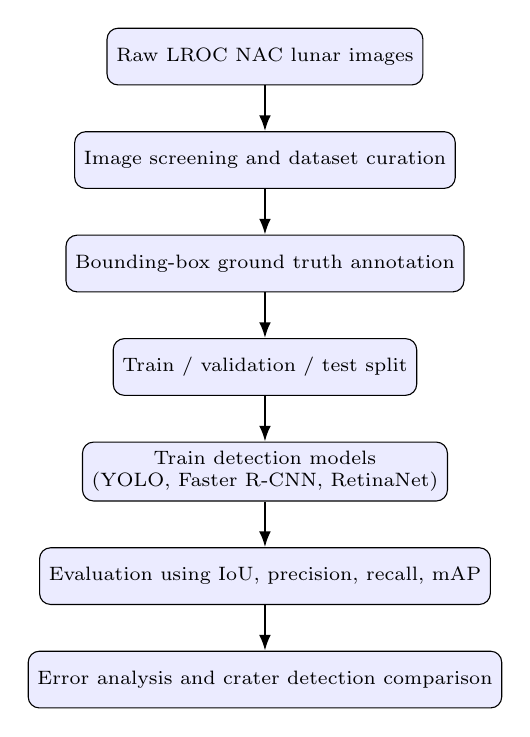
\begin{tikzpicture}[
			node distance=0.58cm,
			every node/.style={font=\scriptsize, align=center},
			block/.style={rectangle, draw, rounded corners, minimum width=3.25cm, minimum height=0.72cm, fill=blue!8},
			line/.style={-{Latex[length=2mm]}, thick}
			]
			
			\node[block] (input) {Raw LROC NAC lunar images};
			\node[block, below=of input] (select) {Image screening and dataset curation};
			\node[block, below=of select] (annotate) {Bounding-box ground truth annotation};
			\node[block, below=of annotate] (split) {Train / validation / test split};
			\node[block, below=of split] (models) {Train detection models\\(YOLO, Faster R-CNN, RetinaNet)};
			\node[block, below=of models] (eval) {Evaluation using IoU, precision, recall, mAP};
			\node[block, below=of eval] (output) {Error analysis and crater detection comparison};
			
			\draw[line] (input) -- (select);
			\draw[line] (select) -- (annotate);
			\draw[line] (annotate) -- (split);
			\draw[line] (split) -- (models);
			\draw[line] (models) -- (eval);
			\draw[line] (eval) -- (output);
		\end{tikzpicture}
		\caption{Draft flowchart of the proposed crater detection project.}
		\label{fig:flowchart}
	\end{figure}
	
	A pseudocode summary of the workflow is:
	\begin{enumerate}
		\item Collect LROC NAC lunar images from multiple regions.
		\item Screen the images for crater visibility and image quality.
		\item Select a realistic subset for manual annotation.
		\item Draw crater bounding boxes and export ground truth labels.
		\item Split the annotated data into training, validation, and test sets.
		\item Train deep learning-based crater detectors.
		\item Evaluate the results using object detection metrics.
		\item Analyze false positives, missed craters, and localization errors.
	\end{enumerate}
	
	\section{Code}
	The project will be implemented in Python. The main software tools will include PyTorch for model development, torchvision or similar libraries for detection model support, OpenCV for image handling and preprocessing utilities, and standard scientific Python packages such as NumPy and Matplotlib for data processing and visualization.
	
	For object detection, the implementation will likely include widely used model frameworks such as YOLO, Faster R-CNN, and RetinaNet. Annotation management and dataset formatting scripts will also be required to connect the ground truth pipeline to the training code.
	
	\section{Deep Learning Detection Methods}
	To detect crater instances in lunar imagery, this project adopts modern deep learning-based object detection approaches. These models learn hierarchical feature representations directly from the data, allowing them to capture crater rims, shadow patterns, circular or elliptical structure, and contextual terrain information.
	
	\subsection{YOLO}
	YOLO is a one-stage object detector that predicts bounding boxes and confidence scores directly from the input image. Its main advantage is computational efficiency, which makes it attractive as a strong baseline method for crater detection. It is particularly useful for large-scale inference, although small and densely clustered craters may remain challenging.
	
	\subsection{Faster R-CNN}
	Faster R-CNN is a two-stage detector that first generates region proposals and then classifies and refines them. This usually improves localization accuracy and can be helpful when crater boundaries are subtle or when multiple crater sizes must be detected in the same image. The trade-off is higher computational cost compared to faster one-stage methods.
	
	\subsection{RetinaNet}
	RetinaNet is another one-stage object detector, but it uses focal loss to handle class imbalance. This is relevant in crater detection because most image regions correspond to background while crater instances occupy a relatively small portion of the image. RetinaNet is therefore a useful comparison model when the imbalance between crater and non-crater regions becomes significant.
	
	In addition to trained detection models, this project will also consider the use of foundation models in inference mode. Models such as Segment Anything (SAM) and Grounding DINO can be used for zero-shot or prompt-based crater detection without task-specific training. These approaches will be explored as a comparison to supervised detectors, particularly to evaluate how well general-purpose vision models can identify crater structures in lunar imagery.
	
	\section{Data Training and Independent Testing Method}
	After annotation, the labeled dataset will be separated into training, validation, and independent testing subsets. Training data will be used to fit the model parameters. Validation data will be used for model selection, hyperparameter adjustment, and early diagnosis of overfitting. The independent test set will remain separate until final evaluation.
	
	This separation is necessary to ensure that the final reported results reflect model generalization rather than memorization of annotated samples. Since the project uses images from multiple lunar regions, care will be taken to maintain diversity across the splits so that evaluation is not biased toward one specific terrain style.
	
	\section{Method Validation Metrics}
	To assess model performance, this project will use standard object detection metrics.
	
	\begin{itemize}
		\item \textbf{Intersection over Union (IoU):} measures how well predicted crater boxes overlap with ground truth boxes.
		\item \textbf{Precision:} measures the fraction of predicted crater detections that are correct.
		\item \textbf{Recall:} measures the fraction of true crater instances that are successfully detected.
		\item \textbf{F1 score:} balances precision and recall.
		\item \textbf{Mean Average Precision (mAP):} summarizes detector performance across confidence thresholds.
	\end{itemize}
	
	In addition to these numerical metrics, qualitative analysis will be performed to examine false positives, missed craters, and localization errors. This is especially important because lunar imagery contains difficult cases where shadows, rough terrain, and crater overlap may confuse the detector.
	
	\section{Bibliography Justification}
	The selected references focus specifically on deep learning approaches for crater detection in planetary imagery. Silburt et al.~\cite{silburt2019lunar} demonstrate that convolutional neural networks can successfully identify lunar craters using learned features. Lee et al.~\cite{lee2020crater} apply CNN-based approaches directly to lunar imagery, improving robustness compared to classical methods. Wang et al.~\cite{wang2022crater} further develops this direction using deep learning-based crater localization ideas that align with object detection.
	
	These works are directly relevant to the proposed project because they establish the effectiveness of deep learning for crater detection and support the use of detection-style learning methods on real lunar imagery.
	
	\section{Links or PDF Documents for the Bibliography}
	The bibliography includes crater-detection-specific papers that can be reviewed alongside the proposal. These references serve as the main literature comparison points for the revised project direction and support the design of the detection task, annotation strategy, and evaluation framework.
	
	\section{Conclusion}
	This proposal outlines a revised crater detection project centered on real lunar imagery, bounding-box ground truth, and deep learning-based object detection. The project moves beyond a purely classical image processing pipeline by incorporating dataset construction, annotation, model comparison, and evaluation. The overall goal is to build a realistic crater detection framework that is technically grounded, aligned with the course, and suitable for evaluation under real lunar imaging conditions.
	
	\bibliographystyle{ieeetr}
	\bibliography{references}
	
	\clearpage
	
	\textbf{Brief Statement of Changes}
	
	Based on the feedback, I clarified and expanded several parts of the project. I added a clearer description of the dataset, including example lunar images and a realistic estimate of about 10 annotated images with multiple crater instances. I also developed a more concrete ground truth approach, including a full annotation pipeline and consistent bounding-box labeling.
	
	I updated the method to focus on deep learning detection instead of just classical techniques, and included multiple models like YOLO, Faster R-CNN, and RetinaNet, along with foundation models for comparison. I also looked into relevant literature (including the Martian project) and added a full pipeline showing how everything connects from data collection to evaluation.
\end{document}